%
After Japan's 2011 earthquake and Fukushima's nuclear power plant disaster, the importance of developing robots capable of helping/replacing humans in dangerous situations or with increased capabilities have raised quickly.
%
This natural disaster showed to the robotics community the lack of case studies that had been conducted towards applications in real case scenarios.
%
Having this as a motivation, in this work we focus on the task of pulling a fire hose by a humanoid robot.
%

Previous works on manipulation tasks by humanoid robots include pushing objects, pivoting, lifting, etc.
%
Hwang et~al. discussed whole body motions of a humanoid robot pushing a wall \cite{pushWall}.
%
Harada et~al. proposed a controller for pushing manipulation by a humanoid robot where the desired trajectory of the ZMP is modified to push an object \cite{pushingZMP}.
%
They also discussed planning the robot's gait in real time to push a heavy object \cite{pushRealTime}.
%
Takubo et~al. discussed pushing a heavy object by a humanoid robot.
The center of mass (CoM) trajectory is modified based on the forces acting on the robot's hands \cite{pushingChair}.
They also discussed a pushing method using multiple contact points between the robot and the object \cite{pushingChair2}.
%
Nozawa et~al. proposed a full-body motion controller for a humanoid robot to push a heavy object by considering the friction forces acting on the robot's arms \cite{pushingForceControl}.
%
Murooka et~al. proposed a whole-body pushing motion by a humanoid robot considering force and balance and using selected contact points with the object to be pushed \cite{pushDesk}.
%
%
Murooka et~al. also discussed the manipulation strategy to use for various objects by a humanoid robot.
The forces applied on the robot are known but not the object dynamical parameters.
Lifting, sliding and tilting the object are the three strategy that are taken into account \cite{Murooka:icra:2014}.
%
Harada et~al. discussed the task of lifting an object and then walk while holding it \cite{heavyObject}.
%

%
\begin{figure}[t]
 \centering
 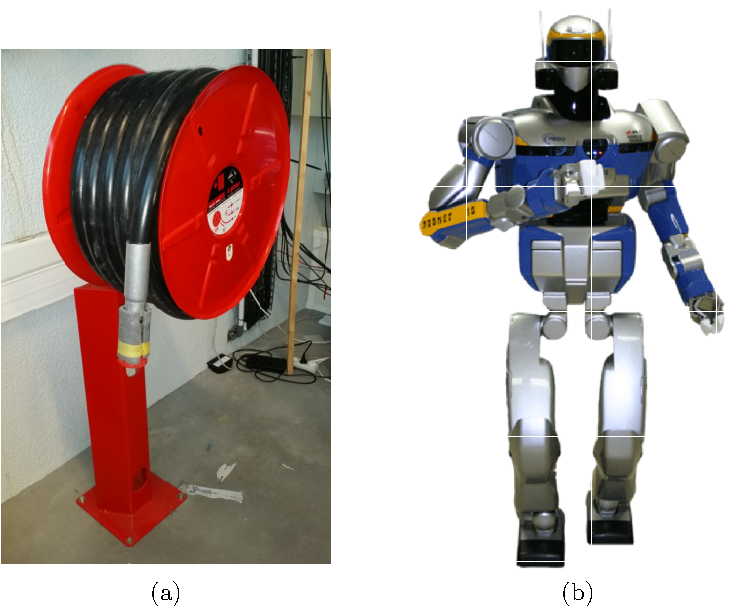
\includegraphics[height=0.40\textwidth]{./figures/Hose_HRP2.pdf}
 \vspace{-3mm}
 \caption{The fire hose is empty and rolled up into a reel used in this work is shown in (a) and the humanoid robot HRP-$2$ is shown in (b).}
 \label{rob_hose}
% \vspace{-5mm}
\end{figure}


%As far as we know, there has been no work on manipulating a fire hose by a humanoid robot.
%
In this work, we discuss the task of picking and then pulling a real fire hose by a humanoid robot while it walks.
%
The fire hose is empty and rolled up into a reel that is fixed to the floor as shown in Fig.~\ref{rob_hose}(a) the nozzle of the hose lays on the floor.
%
A humanoid motion planner is used to generate the picking motion of the humanoid robot HRP-$2$ to avoid any self-collision when the robot leans forward to pick the hose.
%
Then a user friendly walking pattern generator, which input is a velocity relative to the ground plane, is used to generate the walking motion.
%
For pulling the hose a hybrid controller on the robot's wrist holding the hose was implemented.
%
Through simulation analysis it is shown that when the robot is walking while pulling the hose, a drift on the robot's walking direction is generated.
%
A walking task is introduced to correct this drift.
%
Using a motion capture system, the robot's chest position and orientation is tracked in real time.
%
The walking task will compute the desired reference velocity for the robot to arrive to a desired position/orientation.
%
Experimental results confirm the validity of the proposed motion for picking and pulling a fire hose.
%
Moreover we show that the hybrid controller contributes to the improvement of the robot's balance when walking.
%
It must be pointed out that whereas most of the previous work on pushing/pulling is based on force control, in this work we use a combination of position and force control to tackle the drift generated by the fire hose when the robot is walking.


This chapter is organized as follows: 
%
in section \ref{sec_pick} we present the motion planning for the robot to pick the fire hose from the floor.
%
In section \ref{sec_wpg} we briefly introduce the walking pattern generator used in this work.
% 
In section \ref{sec_pull} we show the strategy for a humanoid robot to pull a fire hose and analyze simulation results.
%
In section \ref{sec_wtask} we introduce a walking task to correct the drift in the robot's walking direction generated by the hose.
%
In section \ref{sec_exp} we show the experimental results of the proposed strategy using the HRP-$2$ humanoid robot.
%
Finally, in section \ref{sec_con} we give the conclusion of this work and briefly discuss future work.
